\documentclass[conference]{IEEEtran}
\IEEEoverridecommandlockouts
% The preceding line is only needed to identify funding in the first footnote. If that is unneeded, please comment it out.
\usepackage{cite}
\usepackage{amsmath,amssymb,amsfonts}
\usepackage{graphicx}
\usepackage{textcomp}
\usepackage{fancyhdr}
\usepackage{subfigure}
\usepackage{xcolor}
\usepackage{algorithm}
\usepackage{algorithmic}
\usepackage[a4paper,margin=1in]{geometry}

\def\BibTeX{{\rm B\kern-.05em{\sc i\kern-.025em b}\kern-.08em
    T\kern-.1667em\lower.7ex\hbox{E}\kern-.125emX}}

\pagestyle{fancy}
\fancyhead[L]{Github: 86c6983098ed2410e036cc82cfd861371a7fab92}
\fancypagestyle{firstpage}{%
  \lhead{Github: 86c6983098ed2410e036cc82cfd861371a7fab92}
}

\title{Correlated-Q\\
% {\footnotesize \textsuperscript{*}Note: Sub-titles are not captured in Xplore and
% should not be used}
% \thanks{Identify applicable funding agency here. If none, delete this.}
}

\begin{document}
% \leftmark{github hash: 364e69b8665f1d21354fa25a20ebb4d10bea507f}



\author{\IEEEauthorblockN{Tiantian Guo}
% \IEEEauthorblockA{\textit{dept. name of organization (of Aff.)} \\
% \textit{name of organization (of Aff.)}\\
% City, Country \\
\textit{tguo60@gatech.edu}
}

\maketitle

\thispagestyle{firstpage}

\begin{abstract}
In this project, agents capable of correlated-Q, Foe-Q, Friend-Q and Q-learning~\cite{b1} are developed. The theory of those four algorithms are discussed and an soccer game environment is utilized to implemented the agents. 
\end{abstract}

\begin{IEEEkeywords}
Correlated-Q, Foe-Q, Friend-Q, Q-learning, Soccer Game
\end{IEEEkeywords}

\section{Introduction}

In this project, we extend linear programming (LP) solution for the Nash equilibrum to the environment of soccer game. Four different algorithms: Q-learning, Friend-Q, Foe-Q and Correlated-Q are implemented to estimate the Q-values and value functions $V$. Figure 3 of paper "Correlated-Q Learning"~\cite{b1} is replicated and analyzed.

\section{Reinforcement Learning and Game Theory}

\subsection{Nash Equilibrium}

Nash equilibrium is a set of strategy for a non-cooperative game involving multiple players in which non of the player are better-off by switching to any other strategy, given each player knowing the equilibrium strategy of the other players. For a finite game, there is always at least one Nash equilibrium. Strategy profile $x^* \in S$ is a Nash equilibrium if and only if:
\begin{equation}\label{eq:equilibrium}
\forall i, x_i \in S_i: f_i(x_i^*,x_{-i}^*) \geq f_i(x_i,x_{i-1}^*)
\end{equation}
where $x_i$ is the strategy profile of player $i$ and $x_{-i}$ be the strategy profile for other players. $S = S_1 \times S_2, \times...S_n$ is set of strategy profiles for $n$ players and $f(x) = (f_1(x),f_2(x),...f_n(x))$ is the utility function. 

\subsection{Markov Games and Correlated Equilibrium}

Markov or stochastic games can be visualized as multi-player MDPs and can be represented in form of tupe $I,S,(A_i(s)), P, R_i$, with $I$ as number of players, $S$ as states, $A_i(s)$ as joint action vector for the players, $P$ the probabilistic transition function and $R_i(s,\vec(a)$ as the $i^{th}$ player's reward. Instead of individual player's action, multi-players' actions are considered to be a joint vector for all the players.

The paper presented by Greenwald and Hall~\cite{b1} extends the idea of a multi-agent learning technique to correlated Q-learning. This method generalizes both Nash-Q, Friend and Foe-Q methods~\cite{b2}\cite{b3}. Expanding on Nash-Q algorithm, which is based on Nash equilibrium, learns via a vector of independent probability distributions over actions where all the agents optimize based on each others probabilities. Linear programming is efficient in solving for the correlated equilibrium.

\subsection{Multi-agent Q-Learning}

The strategy selection function $f$ from the algorithm~\ref{al:multiagentQ} is the determining factor for each variant of multiagent Q-Learning. In regular Q-learning, the agents are unaware of the existence of other players, but can observe the state of the game, so every agent just learn its own Q function, thus an agent maximizes values of its own actions max$Q(s,a)$. In friend-Q~\cite{b3}, a particular agent A maximizes its own payoff at each state, and assumes the other players will coordinate their choices to let agent $A$ receive the maximum payoff, thus an agent evaluate state value using max$Q(s,\vec{a}$. Foe-Q~\cite{b3} incorporate mixed strategies for individual actions at Nash equilibrium using maximin algorithm. Correlated-Q(CE-Q) employs mixed strategies for joint actions at correlated equilibrium.

\begin{algorithm}[htb] 
\caption{Multi-agent Q-Learning.} 
\textbf{Input} $f$ - strategy selection function; $\gamma$ - discount; $\alpha$ - learning rate; $D$ - decay; $T$ - total training steps\\
\textbf{Output} action-value function $Q_i^*$;
\begin{algorithmic}[1]\label{al:multiagentQ}
\STATE Initialize $s$ and $Q_1$,...$Q_n$
\FOR{t $\in$ {1,...,T}}
\STATE choose and execute actions $a_1$,...,$a_n$ at state $s$
\STATE observe rewards $R_1$,...,$R_n$ and the next state $s'$
       \FOR{i $\in$ {1,...,n}}
       \STATE $V(s') \leftarrow f_i(Q_1(s'),...,Q_n(s'))$
       \STATE $Q_i(s,a_1,...,a_n \leftarrow (1-\alpha)Q_i(s,a_1,...,a_n)+\alpha[(1-\gamma)R_i + \gamma V_i(s')]$ 
       \ENDFOR
\ENDFOR
\STATE $s \leftarrow s'$
\STATE $\alpha \leftarrow D(\alpha)$
\end{algorithmic}
\end{algorithm}


The update algorithms of Q values are different. Foe-Q updating is based on 
\begin{equation}\label{eq:foe}
V_1(s) = \underset{\sigma_1\in A_1(s)}{\text{max}}\underset{a_2\in A_2(s)}{\text{min}}Q_1(s,\sigma_1,\sigma_2) = -V_2(s)
\end{equation}

Friend-Q updating follows 
\begin{equation}\label{eq:friend}
V_i(s) = \underset{\vec{a}\in A(s)}{\text{max}} Q_i(s,\vec{a})
\end{equation}

CE-Q learning updating is based on 
\begin{equation}\label{eq:ceq}
\sigma \in \text{arg}\underset{\sigma \in \text{CE}}{\text{max}} \sum_{i \in I} \sum_{\vec{a} \in A} \sigma(\vec{a})Q_i(s,\vec{a})
\end{equation}

The intention is to apply these equations on to a special case of Markov Games: Two-Player, Zero-Sum in form of grid soccer and compare how these converge based the error metric in 

\begin{equation}\label{equ:err}
ERR_i^t = |Q_i^t(s,\vec{a}) - Q_i^{t-1}(s,\vec{a})|
\end{equation}

\section{Soccer Game Environment Setup}

The soccer game is a two-player, finite-space zero-sum game. On the grid of 2 rows and 8 columns, there are two players A, B and a ball, as shown in~Fig.\ref{fig:soccer}. The soccer field is a grid. The circle represents the ball. The rules for both player A and B can be summarized as:\par

\begin{enumerate}
  \item The top-left cell is indexed as [0,0] and the bottom-rightcell is indexed as [1,3]. Player A and B are indexed as 0 and 1 respectively. The game is always initiated or reset to state s, as shown in Fig~\ref{fig:soccer}, in which B holds the ball, occupying position $[0,1]$ and A occupies position $[0,2]$.
  \item Each player has five possible actions, stick the ball or go to direction N, S, E, W. The players' actions are executed in random order. Five actions are represented as the two-dimensional movement on the grid: [-1,0] for N, [0,1] for E, [1,0] for S, [0,-1] for west and [0,0] for stick.
  \item At each step of the game, A and B determines their moves simultaneously, but the execution of those two moves are always in random order.
  \item When a player with the ball is trying to move into the position already occupied by the other player, then the ball changes possession, and neither player changes position.
  \item When the ball is in a player's goal, then that player scores $100$, its opponent scores $-100$, and game ends, no matter who has the ball at the time.
  \item After an previous game ends, a new game will be re-initialized to state $s$
\end{enumerate}

\begin{figure}[htbp]
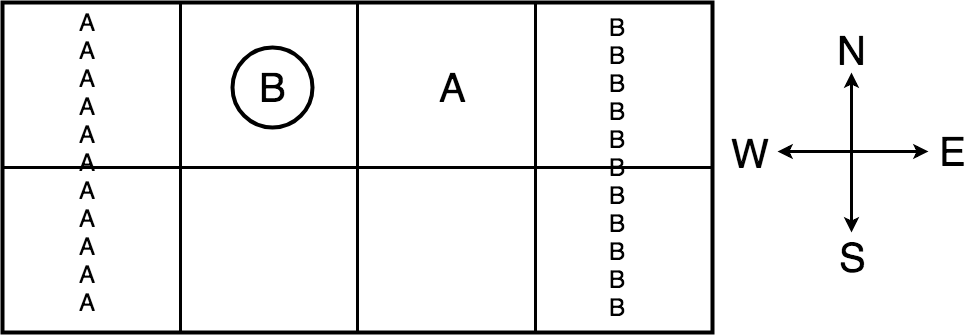
\includegraphics[width=\linewidth]{soccer.png}
\caption{Soccer Game. State $s$.}
\label{fig:soccer}
\end{figure}

\begin{algorithm}[htb] 
\caption{Soccer game environment.} 
\textbf{Input} Current positions, ball possession and new actions from players A and B;\\
\textbf{Output} A state, B state, ball possession, scores, done;
\begin{algorithmic}[1]\label{al:soccer}
\STATE Init scores
\STATE Check input actions and randomly decide sequence of movement of A and B
\STATE First mover moves
\IF{collision}
\STATE check ball status and exchange possesion
\ELSE
\STATE update positions of first mover
       \IF{GOAL for any players}
       \STATE update scores, done=1, return
       \ENDIF
\ENDIF
\STATE Second mover moves
\IF{collision}
\STATE check ball status and exchange possesion, return
\ELSE
\STATE update positions of second mover
       \IF{GOAL for any players}
       \STATE updage scores, done=1, return
       \ENDIF
\ENDIF
return A state, B state, ball posession, scores, done
\end{algorithmic}
\end{algorithm}

The algorithm~\ref{al:soccer} illustrates the implementation of the soccer game environment. The environment takes in current positions of both players, ball possession and new action selections from player A and B. It first checks whether teh input actions are in valid range, then randomly decides either A or B to take the first move. The first mover performs the action and the collision checking mechanism decides whether there is a change of ball. It then checks whether the player has scored for himself or the opponent. After the first mover finishes his step, if there is no goal, the second mover performs teh action and goes through teh same process. The step update finishes and returns to the caller for the updated states of two players, scores and game termination flag.

\section{Experiments and Results}\label{sec:results}

Experiments represented in Fig 3 in \cite{b1} were replicated to show $ERR_i^t$ across 1 million training steps for Q-learning, friend-Q, foe-Q and CE-Q on soccer environment using different parameters, and their results and performances were compared. The Q values at a particular state action pair for player A, Q(state=$s$,action=$S$) is recorded during training iterations.

All four training algorithms are tested with $\epsilon$-greedy with $\epsilon$: 1 $\to$ 0.001 with the $\epsilon$ decay rate as 0.999995, discount $\gamma$ = 0.9, leanring rate $\alpha$ from 1.0 $\to$ 0.001 with the $\alpha$ decay rate as 0.999995 or 0.99. The y axis in left two figures are limited to 0.5 and there is no y axis uplimit in right two figures. 

\subsection{Q-learning}

In Q-learning, the two agents are not aware of the actions taken by their opponents, however they can observe the state of the game. Player A can observe position of B, as well as possession of the ball, vice versa. Since a player is only aware of its own action, it simply choose the action with the largest Q value at the particular state to evaluate the utility of that state.

\begin{figure}[htbp]
\centering
\subfigure[Zoom in]{
\begin{minipage}[t]{0.48\linewidth}
\centering
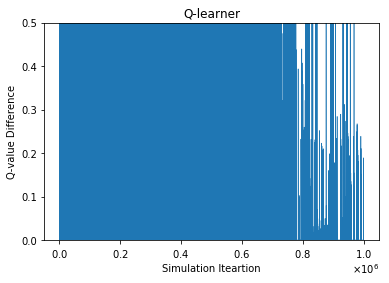
\includegraphics[width=1.5in]{Q1.png}
%\caption{fig1}
\end{minipage}%
}%
\subfigure[Zoom out]{
\begin{minipage}[t]{0.48\linewidth}
\centering
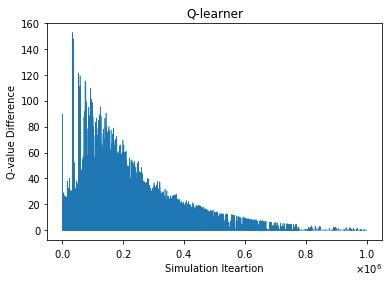
\includegraphics[width=1.5in]{Q2.png}
%\caption{fig2}
\end{minipage}%
}%
\centering
\caption{$\alpha$ decay: 0.999995}
\label{fig:QLearning1}
\end{figure}

\begin{figure}[htbp]
\centering
\subfigure[Zoom in]{
\begin{minipage}[t]{0.48\linewidth}
\centering
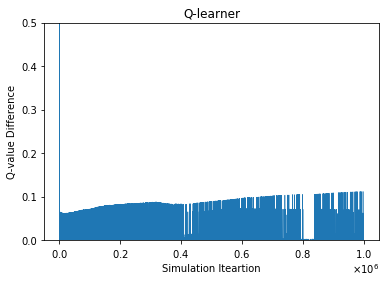
\includegraphics[width=1.5in]{Q3.png}
%\caption{fig1}
\end{minipage}%
}%
\subfigure[Zoom out]{
\begin{minipage}[t]{0.48\linewidth}
\centering
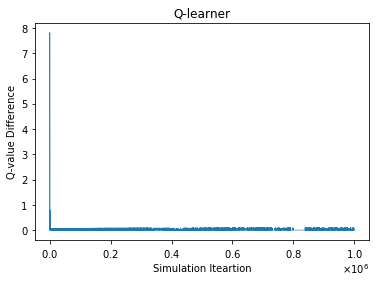
\includegraphics[width=1.5in]{Q4.png}
%\caption{fig2}
\end{minipage}%
}%
\centering
\caption{$\alpha$ decay: 0.99}
\label{fig:QLearning2}
\end{figure}

The effect of $\alpha$ decay rate is shown in Fig.~\ref{fig:QLearning1} and~\ref{fig:QLearning2}. The left figure in Fig~\ref{fig:QLearning1} almost replicates the figure (d) in Fig.3 in paper~\cite{b1}. But the figures are not exactly the same due to the different selections of hyperparameters like $\gamma$, $\epsilon$, $\alpha$, $\alpha$ decay etc. As we can see the plot difference between $\alpha decay = 0.999995$ and $\alpha decay = 0.99$. $\alpha$ decay 0.999995 performs better than $\alpha$ decay 0.99. The plot from $\alpha$ decay 0.99 does not show any convergence trend at all. As long as we try various combination of{} hyperparameters, we can achieve same plot as in~\cite{b1}.

Q-learning algorithm results do show a decreasing trend but even after million iterations it does not fully converge.

\subsection{Friend-Q}

In friend-Q, a player, A, is aware of actions of all players, as well as the full state of game, however in evaluating the utility of a particular state, it chooses the joint action with the highest Q value, and assumes its opponent will cooperate and let it choose that joint action. The opponent behaves the same, assuming A will cooperate with it.

\begin{figure}[htbp]
\centering
\subfigure[Zoom in]{
\begin{minipage}[t]{0.48\linewidth}
\centering
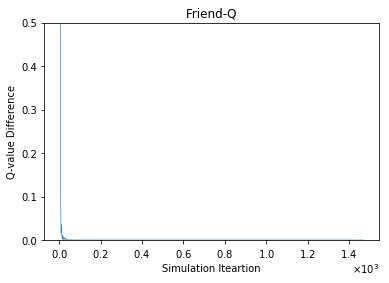
\includegraphics[width=1.5in]{FQ1.png}
%\caption{fig1}
\end{minipage}%
}%
\subfigure[Zoom out]{
\begin{minipage}[t]{0.48\linewidth}
\centering
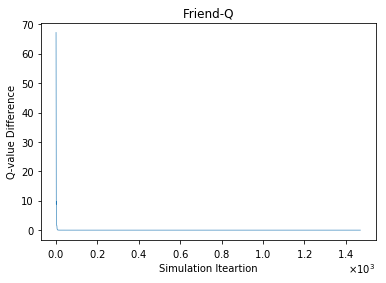
\includegraphics[width=1.5in]{FQ2.png}
%\caption{fig2}
\end{minipage}%
}%
\centering
\caption{$\alpha$ decay: 0.999995}
\label{fig:FQ1}
\end{figure}

\begin{figure}[htbp]
\centering
\subfigure[Zoom in]{
\begin{minipage}[t]{0.48\linewidth}
\centering
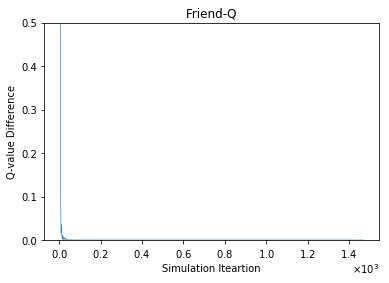
\includegraphics[width=1.5in]{FQ3.png}
%\caption{fig1}
\end{minipage}%
}%
\subfigure[Zoom out]{
\begin{minipage}[t]{0.48\linewidth}
\centering
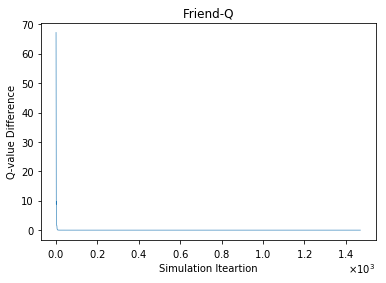
\includegraphics[width=1.5in]{FQ4.png}
%\caption{fig2}
\end{minipage}%
}%
\centering
\caption{$\alpha$ decay: 0.99}
\label{fig:FQ2}
\end{figure}

In Fig~\ref{fig:FQ1} and~\ref{fig:FQ2}, the effect of $\alpha$ decay is minimal to the Q value difference. Only first 1500 iterations are shown in the graph. It demonstrates a very fast convergence of the Q-value. The graph closely resembles the shape in Greenwald's paper~\cite{b1}, though the original paper it takes more steps for convergence. Some hyperparamters combinations might achieve the exact shape and the same number of converge iterations.


\subsection{Foe-Q}

In foe-Q, each agent tries to maximize its own reward and minimize its opponents, and the utility of a particular state $V(s)$ is evaluated to be opposite for the two players. 

\begin{figure}[htbp]
\centering
\subfigure[Zoom in]{
\begin{minipage}[t]{0.48\linewidth}
\centering
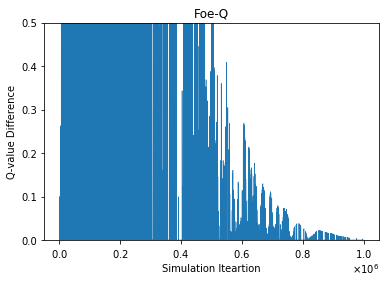
\includegraphics[width=1.5in]{FoQ1.png}
%\caption{fig1}
\end{minipage}%
}%
\subfigure[Zoom out]{
\begin{minipage}[t]{0.48\linewidth}
\centering
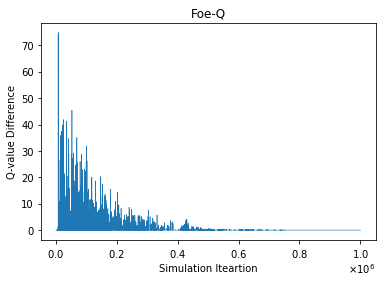
\includegraphics[width=1.5in]{FoQ2.png}
%\caption{fig2}
\end{minipage}%
}%
\centering
\caption{$\alpha$ decay: 0.999995}
\label{fig:FoQ1}
\end{figure}


\begin{figure}[htbp]
\centering
\subfigure[Zoom in]{
\begin{minipage}[t]{0.48\linewidth}
\centering
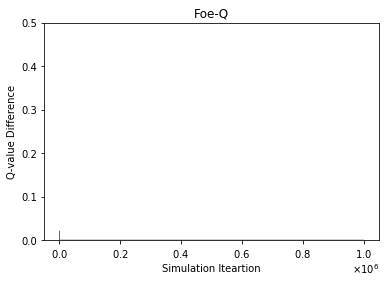
\includegraphics[width=1.5in]{FoQ3.png}
%\caption{fig1}
\end{minipage}%
}%
\subfigure[Zoom out]{
\begin{minipage}[t]{0.48\linewidth}
\centering
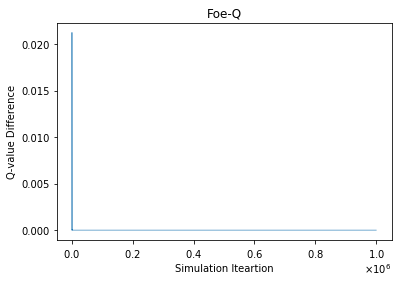
\includegraphics[width=1.5in]{FoQ4.png}
%\caption{fig2}
\end{minipage}%
}%
\centering
\caption{$\alpha$ decay: 0.99}
\label{fig:FoQ2}
\end{figure}

The graph replicates Fig 3 in Greenwald's paper~\cite{b1}, in our replication, the graph begins to converge at around 800,000 steps while in~\cite{b1}, the graph converges at around 700,000 iterations. As the maxmin (Foe-Q) algorithm requires an linear programming solver to calculate value function and probability distribution over actions, different solver used might contribute to such difference.

\subsection{Correlated-Q}

CE-Q evaluates the utility at a particulate state $V(s)$ using the mixed strategy of joint actions obtained at a correlated equilibrium. CE-Q learner learns two separate Q tables for players A and B, and using Q values from both tables to generate a strategy of joint actions using linear programming. 

\begin{figure}[htbp]
\centering
\subfigure[Zoom in]{
\begin{minipage}[t]{0.48\linewidth}
\centering
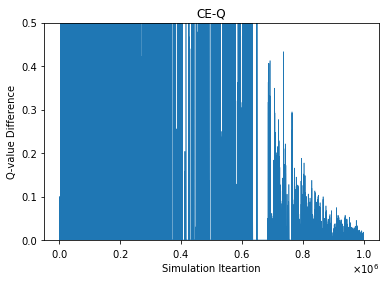
\includegraphics[width=1.5in]{CE1.png}
%\caption{fig1}
\end{minipage}%
}%
\subfigure[Zoom out]{
\begin{minipage}[t]{0.48\linewidth}
\centering
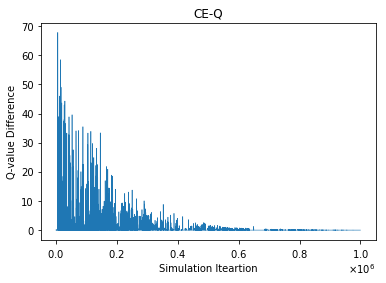
\includegraphics[width=1.5in]{CE2.png}
%\caption{fig2}
\end{minipage}%
}%
\centering
\caption{$\alpha$ decay: 0.999995}
\label{fig:CE1}
\end{figure}


\begin{figure}[htbp]
\centering
\subfigure[Zoom in]{
\begin{minipage}[t]{0.48\linewidth}
\centering
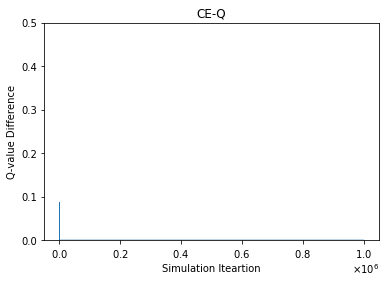
\includegraphics[width=1.5in]{CE3.png}
%\caption{fig1}
\end{minipage}%
}%
\subfigure[Zoom out]{
\begin{minipage}[t]{0.48\linewidth}
\centering
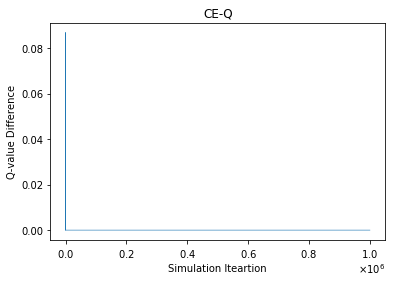
\includegraphics[width=1.5in]{CE4.png}
%\caption{fig2}
\end{minipage}%
}%
\centering
\caption{$\alpha$ decay: 0.99}
\label{fig:CE2}
\end{figure}

Fig~\ref{fig:CE1} and~\ref{fig:CE2} shows $ERR_i^t$ for Foe-Q algorithm across 1 million iterations. It shows a decreasing Q-value difference at state $s$, indicating the convergence of the algorithm. Moreover, the graph closely resemble the graph of Foe-Q in terms of convergence. There are few factors contributing to this observation. First, soccer game is a zero-sum finite-space game, hence different CE-Q algorithms will generate same values for all equilibria. Secondly, as explained in the original paper, CE-Q learns the same set of Q-values as Foe-Q. The difference of graphs generated in this report and in the paper~\cite{b1} might result from the use of different linear programming solver and hyperparameter selections.

\section{Conclusion}

The details on game theory foundation from nash equilibrium and correlated equilibrium to the generalization of MDP as markov games are explained. This report implemented four multi-agent Q learning algorithms: Q-Learning, Friend-Q, Foe-Q and CE-Q in the soccer game environment. The error differences plots are compared with the results shown in~\cite{b1}. Deeper understanding is gained on Markov Games and CE-Q.

\begin{thebibliography}{00}{}
\bibitem{b1} Greenwald, A., and Hall, K., Correlated-Q learning \textit{International Conference on International Conference on Machine learning}, 2003.
\bibitem{b2} Junling Hu, Michael P. Wellman, Nash Q-Learning for General-Sum Stochastic Games \textit{Journal of Machine Learning Research}, 4, 1039-1069, 2003.
\bibitem{b3} Michael L. Littman, Friend-or-Foe Q-learning in General-Sum Games \textit{ICML}, 322-328, 2001.
\end{thebibliography}
\vspace{12pt}

\end{document}
